\documentclass[border=.2cm]{standalone}
\usepackage{tikz}
\usepackage{amsmath}
\usetikzlibrary{angles}

\begin{document}

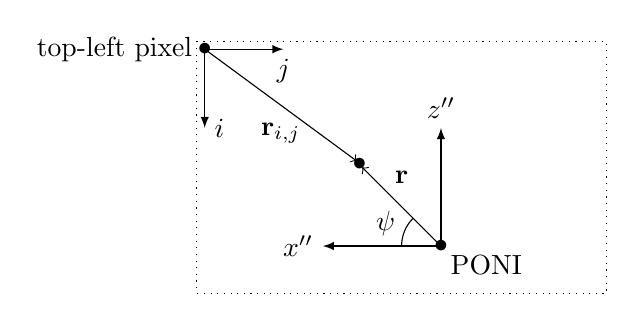
\begin{tikzpicture}
    \draw[->,>=latex] (0,0) coordinate(O) node[anchor=east,xshift=-1] {top-left pixel} -- (1,0) node[anchor=north] {$j$};
    \draw[->,>=latex] (O) node[] {$\bullet$} -- (0,-1) node[anchor=west] {$i$};
    \draw[dotted] (-0.1,.1) -- (5.1,.1) -- (5.1,-3.1) -- (-.1,-3.1) -- cycle;
    \draw[->,>=latex] (3,-2.5) coordinate(O2) node[anchor=north west] {PONI} -- ++ (-1.5,0) coordinate (y) node[anchor=east] {$x''$};
    \draw[->,>=latex] (O2) node[] {$\bullet$} -- ++ (0,1.5) coordinate(z) node[anchor=south] {$z''$};
    \draw[->] (O2) -- ++ (-1, 1) coordinate(r) node[midway,above,yshift=5] {$\mathbf{r}$};
    \draw pic [draw,angle radius=0.5cm] {angle = r--O2--y};
    \node[xshift=-1,yshift=1] at (r) {$\bullet$};
    \node[above,xshift=-20] at (O2) {$\psi$};
    \draw[->] (O) --++ (1.93,-1.42) node[midway, below,yshift=-3] {$\mathbf{r}_{i,j}$};
\end{tikzpicture}

\end{document}